\chapter[Características Fractales del Pan]{Características Fractales y Multifractales del Pan}

%\subsection{Características Fractales y Multifractales del Pan}
En esta sección nos proponemos caracterizar distintas muestras de pan por medio de extracción de características.
Gracias a estas t\'ecnicas, podemos validar los resultados obtenidos en los cap\'itulos anteriores con una base matem\'atica s\'olida, m\'as all\'a de la validaci\'on visual realizada por las personas, la cual es utilizada tradicionalmente en computaci\'on gr\'afica.
Además, las características fractales y multifractales capturan características esenciales que pueden ser utilizadas para la clasificación de las muestras, superando a otros clasificadores del estado del arte.

\section{Introducción}

Existen diversos criterios para evaluar la fidelidad de las im\'agenes resultantes. Uno de ellos consiste en realizar pruebas con personas, entreg\'andoles im\'agenes verdaderas y sint\'eticas, sin que ellas sepan a cu\'al categor\'ia pertenece cada una, pidi\'endoles que clasifiquen las im\'agenes en verdaderas y sint\'eticas. Si las im\'agenes sint\'eticas resultan ser clasificadas en un porcentaje adecuado como reales, se puede considerar al experimento como satisfactorio.

Otro m\'etodo consiste en comparar las im\'agenes por medio de extracci\'on de caracter\'isticas. En el presente trabajo se comparan dimensiones fractales (DF) de determinadas caracter\'isticas de muestras reales y sint\'eticas. Para ello se utilizan las DFs de Korcak \cite{Mandelbrot83} y la dimensi\'on Box \cite{Peitgen2004}.


One of the most important factors to evaluate the quality of a bread loaf is related to its crumb structure. Close examination of different slices reveals considerable variation in the cell (air bubble) size even within a single sample of the same bread type. 

Fractal and multifractal analysis of images have pro\-ved to be able to capture useful properties of the underlying material being represented. These features have been successfully applied in different areas, such as medi\-cine \cite{Andjelkovic2008,Yu2011} and texture classification \cite{Wendt2009}. In food research, fractal and multifractal analysis has been applied in the study of apple tissues \cite{Mendoza2010}, pork sirloins \cite{Serrano2012}, and also in chocolate, potato and pumpkin surfaces \cite{Quevedo2002}. Through several procedures \cite{Peitgen2004,Gonzales2008}, it is possible to obtain different Fractal Dimensions (FD), each of them capturing a different property of the material ({\em e.g.}, porosity, rugosity).

Data analysis of the results of the feature extraction process is useful for obtaining key properties of materials. This information could then be used in quality measurements of real samples and in the validation of synthetic representations of them. In other words, these processes are useful to determine if a given image presents the observed features in that material, allowing to associate quality measure parameters to it. In~\cite{Fan2006}, a bread crumb quality test based on Gabor filters was performed, obtaining good results. Nevertheless, a small database was used ($30$ images). In \cite{Gonzales2008} several fractal features were obtained for one type of bread, demonstrating that a vector of FDs would be capable of obtaining key features of the crumb texture more accurately than using a single FD.

In this work we propose the application of the Multifractal Spectrum (MFS) to describe and classify different bread crumb types. One of the main features of the MFS is its bi-Lipschitz invariance, that is, invariance to perspective transforms (viewpoint changes) and smooth texture surface deformations. It is shown that the MFS is also locally invariant to affine changes in illumination. These features are useful to describe bread crumb structures in a robust way that results adequate for the purposes of this study.

Food classification has already been applied using fractal and other techniques in \cite{Zong2010,Bosch2011} but these works do not address the intra-class problem, {\em i.e.}, the classification is made among different foods and not by making different classes out of the same food.

In a previous work \cite{Baravalle2012_2}, we showed that the MFS in combination with other fractal features was able to classify different bread crumb types with high accuracy. The present work aims to simplify the model and strengthen these results by comparing {\em only} the MFS with other state-of-the-art features and using different classifiers, and also to study the correlations of the features obtained with the procedure and different texture features obtained from the images (see next sections).

The proposed method is compared to other state-of-the-art features for texture classification. The results of this feature extraction procedure show that the classifier is robust and presents good discrimination properties to distinguish between different bread types and also bread from non bread images.

En \cite{Gonzales2008} se present\'o un trabajo de c\'alculo de distintas DFs sobre muestras de pan. Las mismas son obtenidas a trav\'es de algoritmos diferentes a los utilizados en este trabajo. Los resultados obtenidos no tienen en cuenta la posibilidad de estimar m\'as de una DF para las muestras.


\subsection*{Dimensi\'on Box}
La misma intenta simplificar el c\'alculo de la DF de Hausdorff, debido a que \'esta resulta muy dif\'icil de obtener \cite{Peitgen2004} (o imposible si el objeto no es estrictamente autosimilar).

Dada una imagen, se la subdividide en una grilla $M\times M$ donde el largo del lado de cada cuadrado formado es $\delta$. Si $N(\delta)$ representa el n\'umero de cuadrados que contienen al menos un p\'ixel resultado de una binarizaci\'on de la imagen (p\'ixel blanco) para ese $\delta$, la dimensi\'on Box $D_{b}$ queda definida como:\\

$D_{b} = \displaystyle\lim_{\delta \to 0}{\frac{\log(N(\delta))}{\log (1/\delta)}}$\\

En el algoritmo resultante se utiliza una imagen binarizada de la original. A partir de ella se seleccionan distintos $\delta$, realizando un conteo de cuadrados que contienen p\'ixeles blancos en cada caso (para evitar inestabilidad num\'erica, se utiliza un promedio de casos, estableciendo distintas posiciones de la grilla sobre la imagen). Finalmente se realiza un ajuste por regresi\'on lineal de los datos obtenidos en el espacio $\log-\log$, cuya pendiente es por definici\'on la DF Box de la imagen.

\subsection*{Dimensi\'on Fractal de Korcak}
Esta DF fue introducida en \cite{Mandelbrot83}, basada en un trabajo previo del cient\'ifico checo Kor$\check{c}$\'ak. La misma funciona como un descriptor de fragmentaci\'on de objetos en dos dimensiones. Su definici\'on formal es la siguiente \cite{Imre11}:

$N(A > a) = k a^{-K},$

\noindent
donde K es el exponente Korcak de fragmentaci\'on (patchiness), N es el n\'umero de fragmentos cuyo \'area $A$ es mayor que el valor $a$, y $k$ es una constante. La DF de Korcak, $D_{k}$, queda definida de la siguiente manera:

$K = D_{k}/2.$

El procedimiento para calcular $D_{k}$ consiste en ajustar una recta a partir de pares $(\log(a),\log(N))$. En este trabajo se considera apropiado este valor dado que las muestras de pan est\'an compuestas por burbujas de distinto tama\~no, resultantes del proceso de cocci\'on del mismo, por lo tanto, se busca que las muestras sint\'eticas posean caracter\'isticas similares de {\em fragmentaci\'on}.

\subsection*{Segmentaci\'on de las Im\'agenes}
La imagen original es binarizada utilizando el algoritmo de Otsu \cite{Otsu79} para definir un valor de umbral, a partir del cual se decide si el p\'ixel ser\'a negro o blanco en la binarizaci\'on. 

Un error muy com\'un utilizando este m\'etodo es que muchas regiones de la imagen donde el ojo detecta masa, son consideradas burbujas (color blanco). En estos casos se obtuvo un mejor resultado al definir un umbral $t$ para una imagen determinada (observando el resultado para cada imagen). La misma es transformada a escala de grises y se establece como burbuja a cualquier valor menor a $t$. En casos donde este procedimiento no resulta satisfactorio, se elige una subregi\'on de la imagen donde el algoritmo de segmentaci\'on presenta buenos resultados.


A modo de ejemplo, en la Figura \ref{bin} puede observarse una imagen y su binarizaci\'on.

\begin{figure}
\centering
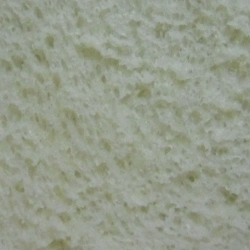
\includegraphics[width=5cm]{figures/lactal}
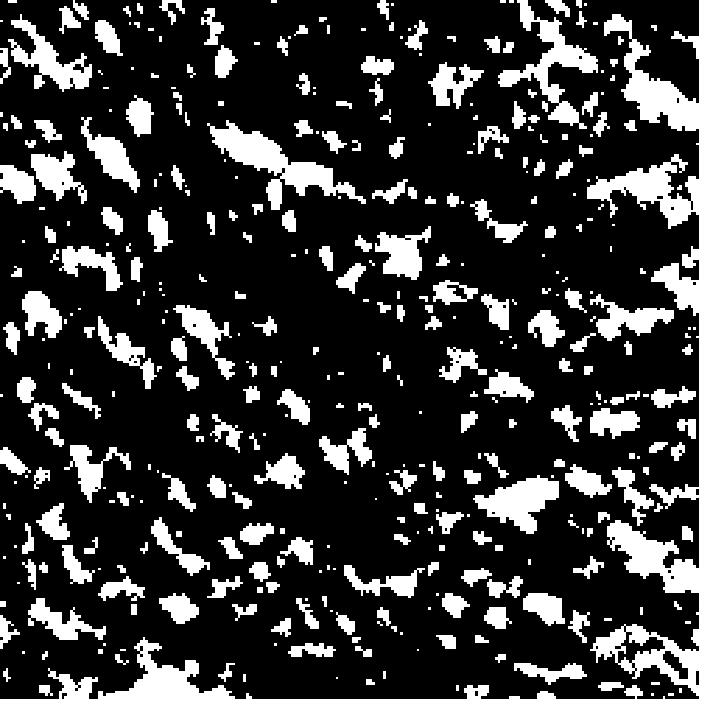
\includegraphics[width=5cm]{figures/lactalBin}
\caption{Imagen y su binarizaci\'on}
\label{bin}
\end{figure}


En la Figura \ref{fitbox} se observan los valores obtenidos en el c\'alculo de la dimensi\'on Box para esta imagen y la recta que ajusta estos valores. 

\begin{figure}
\centering
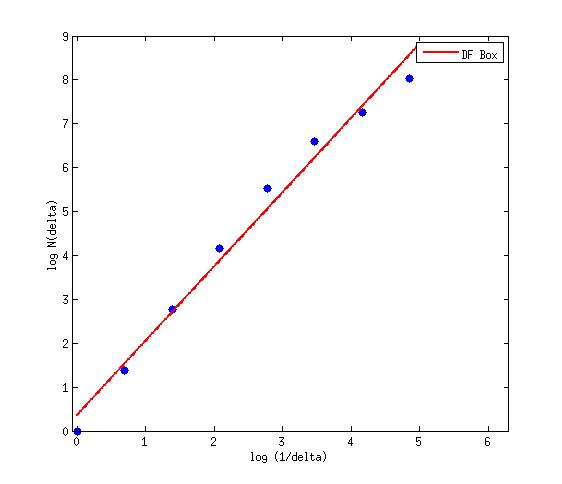
\includegraphics[width=8cm]{figures/fitbox}
\caption{Dimensi\'on Box de la imagen de la Figura \ref{bin}}
\label{fitbox}
\end{figure}


En la Figura \ref{fit} se observan los valores obtenidos por el algoritmo de Korcak para esta imagen y las rectas aproximantes (en la siguiente secci\'on se explica el por qu\'e de dos rectas aproximantes).

\begin{figure}
\centering
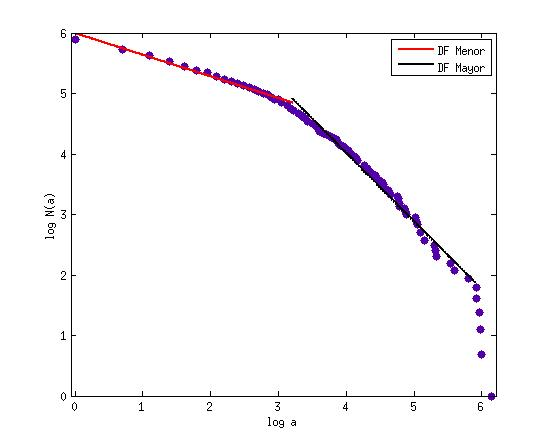
\includegraphics[width=8cm]{figures/lactal1PlotKorcak}
\caption{DFs de Korcak de la imagen de la Figura \ref{bin}}
\label{fit}
\end{figure}

\subsection*{Dimensiones Estimadas}

En los diagramas $\log-\log $ obtenidos por el algoritmo (Korcak), puede observarse que una \'unica recta no ajusta correctamente los valores. Esto sugiere que las muestras presentan caracter\'isticas {\em multifractales} \cite{Mandelbrot89}. Es decir que es posible calcular m\'as de una DF para la misma imagen. Se realizaron pruebas con pan lactal y mignon. Las DFs encontradas se incluyen en la Tabla \ref{tab:korcak}.\\

\begin{table}
\center
\begin{tabular}{|| l | l | l ||}
    \hline
     & DF (menor) & DF (mayor) \\    
    \hline
    Lactal 1 & 0.7152 & 2.214 \\
    \hline
    Lactal 2 & 0.8638 & 2.182 \\
    \hline
    Lactal 3 & 0.7598 & 2.046 \\
    \hline
    Lactal 4 & 0.8656 & 2.598 \\
    \hline
    Mignon 1 & 0.5068 & 1.1452\\
    \hline
    Mignon 2 & 0.4214 & 1.1608\\
    \hline
\end{tabular}
\caption{DFs de Korcak estimadas en muestras reales de pan}
\label{tab:korcak}
\end{table}

Puede observarse que para distintos tipos de panes las DFs resultantes var\'ian de manera considerable, por lo cual es posible pensar a estas DF como clasificadores de muestras.

Para la regresi\'on por DF Box, los valores que se obtuvieron se muestran en la Tabla \ref{tab:box}.

\begin{table}
\begin{center}
\begin{tabular}{|| l | l | l ||}
    \hline
     & DF \\    
    \hline
    Lactal 1 & 1.692 \\
    \hline
    Lactal 2 & 1.761 \\
    \hline
    Lactal 3 & 1.743\\
    \hline
    Lactal 4 & 1.73 \\
    \hline
    Mignon 1 & 1.686 \\
    \hline
    Mignon 2 & 1.726 \\
    \hline
\end{tabular}
\caption{DFs Box estimadas en muestras reales de pan}
\label{tab:box}
\end{center}
\end{table}

Se observa cierta similitud entre los valores obtenidos, por lo cual resulta un par\'ametro \'util el cual deben cumplir las im\'agenes sint\'eticas. Sin embargo no resulta un par\'ametro adecuado para realizar clasificaci\'on de muestras.


\section{Clasificación de Imágenes de Pan Utilizando Características Fractales y Multifractales.}



En esta sección realizaremos una extracción de características útiles sobre la miga de pan, la cual nos permitirá caracterizar la miga y validar los resultados obtenidos.


Se obtuvieron $20$ imágenes de $4$ tipos de panes diferentes ({\em baguette}, {\em lactal}, {\em salvado} y {\em sandwich}, contabilizando $80$ imágenes) utilizando un escáner HP PSC 1210 con los siguientes parámetros de captura:  highlight $190$, shadows $40$, and midtones $1$. Las imágenes fueron obtenidas a una resolución de $380\times 380$ píxeles (el área máxima posible para los $4$ tipos de pan) a una resolución de $350$ dpi ($1$ pixel $= 0.00527$ $[mm^{2}]$). Las mismas fueron convertidas a escala de grises ($8$ bits). Además, se obtuvieron $20$ imágenes de cada tipo de pan utilizando una cámara digital con la misma resolución espacial. Las condiciones de iluminación de estas imágenes son distintas a las de las imágenes del escáner para probar la robustez del método. En la FIgura ~\ref{fig:camera} se observan $4$ ejemplos de imágenes de pan obtenidas con la cámara digital. Además se utilizaron $40$ imágenes de la base de imágenes CalTech101 dataset~\cite{FeiFei04} para introducir imágenes de objetos diferentes al pan y observar la capacidad del método para separar panes de otros objetos.

\subsection{Extracción de Características de Migas de Panes}
Para comprender mejor los valores devueltos con las dimensiones obtenidas, se extrajeron características típicas de las imágenes binarizadas para establecer correlaciones con las dimensiones multifractales.

Se computaron la fracción de vacío de la imagen (FV), el área media de las burbujas (MCA) y el desvío estándar del área media de las burbujas (stCA) para establecer relaciones con la porosidad, granularidad y heterogeneidad de las diferentes migas.

\subsubsection{Binarización de migas de pan utilizando umbralamiento local}
Para determinar las mismas, sólo se utilizaron imágenes binarizadas de las muestras tomadas con el escáner, evitando mezclar imágenes tomadas en diferentes condiciones lumínicas. Las binarizaciones se llevaron a cabo utilizando el algoritmo de umbralamiento local descripto en \cite{White83}. El mismo presentó mejores resultados que la utilización del algoritmo presentado en \cite{Huang95} y utilizado en \cite{Gonzales2008}, el cual utiliza un umbralamiento global de la imagen. Esto se debe a que sutilies variaciones en la iluminación de la misma muestra resultados incorrectos en la determinación de burbujas. En la Figura~\ref{fig:bread} se observa una imagen de cada tipo de pan (primera fila) y su binarización correspondiente utilizando el algoritmo descripto (segunda fila). Elementos pequeños de la imagen de $1$ o $2$ píxeles fueron removidos utilizando una operación de {\em opening} (erosión y dilatación) con un elemento estructurante de $2\times 2$. Este método presenta buenos resultados incluso con condiciones de iluminación variando sobre la imagen.

En cada píxel, el resultado de la binarización se computa a través de un promedio de los niveles de gris en una ventana que rodea ese píxel. Este promedio se compara con un umbral definido por el nivel de gris del píxel actual multiplicado por un número de bias y en caso de ser mayor, el píxel resultará blanco (en otro caso, negro), es decir:
\begin{equation}
\frac{\sum_{x,y \in W} f(x,y) }{W_{size}} \geq f(x_{c},y_{c}) \times bias,
\label{eqn:white}
\end{equation}
donde $x_{c},y_{c}$ son las coordenadas del píxel actual y  $W$ es la ventana que rodea al píxel. Los dos parámetros que definen al algoritmo son: el tamaño de la ventana ($W_{size}$) y el $bias$. 

Experimentalmente encontramos que estos parámetros dependen del método de captura utilizado. Los mejores valores para las muestras de escáner fueron $80$ para el tamaño de la ventana y $1.15 $ para el bias. En el caso de las muestras tomadas con una cámara digital, los valores óptimos fueron $80$ para la ventana y $1$ para el bias.  Estas diferencias parecen ser causadas por las diferentes condiciones de iluminación presentes en las imágenes. Queda planteado como trabajo a futuro la determinación automática de estos parámetros.

\section{MFS como vector de caracter\'isticas}

En esta sección nos proponemos mostrar el comportamiento adecuado del MFS como descriptor de imágenes de pan, el cual es capaz de distinguir estas de otros objetos.

Computamos el MFS para cada una de las $200$ imágenes presentes en la base de datos ($40$ imágenes de cada tipo, incluyendo no-pan), obteniendo $5$ clases balanceadas.  Las siguientes subsecciones analizaremos los datos obtenidos, además de utilizarlos en la clasificación de las muestras.

\subsection{Análisis del MFS de las imágenes de pan y no-pan}

Los Mapas Auto-organizados ( Self-organising maps -  SOM)~\cite{Kohonen2001} son herramientas de aprendizaje no supervisado que permiten reducir la dimensionalidad de un conjunto de datos para entender mejor su relación espacial. Los mapas SOM mapean datos multidimensionales en $2$ dimensiones utilizando información de vecindad, preservando así la información topológica de los mismos.

La Figura~\ref{fig:somfractal} muestra el  SOM de las representaciones multifractales de las imágenes de pan y de no-pan en una grilla de $10\times 10$ (el comportamiento es similar para distintos tamaños de grilla). La imagen de la izquierda muestra las $5$ clases ({\em baguette}, {\em lactal}, {\em salvado}, {\em sandwich} y {\em no-pan}). En la imagen de la derecha la clase {\em no-pan} fue quitada y el SOM recomputado para las restantes $4$ clases con la intención de observar mejor la relación entre los MFS de las distintas clases de pan. Las imágenes muestran clases fácilmente separables a primera vista. Un clasificador podría determinar regiones del espacio y clasificar de manera adecuada las clases, ya que se encuentran claramente separadas unas de otras (no existen prácticamente celdas con más de un número de clase en ellas).

En la Figura~\ref{fig:boxplotsMFS}, se muestran boxplots de los cuatro tipos de panes con la media de cada dimensión (en rojo) unida por una línea a trozos. Cada dimensión fractal corresponde a un valor de $\alpha_{i}$. En nuestros experimentos el vector de MFS contiene $20$ dimensiones fractales. De estos datos se infiere que la primer mitad del MFS () (primeras $10$ DFs, $\alpha \in [0,0.53)$), la dispersión es mayor que en la segunda mitad del espectro  (últimas $10$ DFs, $\alpha \in [0.53,1]$). Es decir, la segunda mitad del espectro puede ideitificar mejor cada tipo de pan.

Los datos muestran que cada tipo de pan posee una curva característica en este sector del espectro, pero esta curva se modifica si se modifican las condiciones de iluminación (es decir, si se toma con el escáner o la cámara), en otras palabras esto altera el MFS obtenido, y por lo tanto no poseemos un único MFS para cada tipo de pan. 

Por completitud, en la Figura~\ref{fig:meansMFS}, mostramos la media y el desvío estándar del MFS de cada tipo de pan. La imagen muestra, al igual que en los casos anteriores, el MFS puede ser aprovechado para separar diferentes tipos de pan, ya que los valores medios de cada clase son distintos.

\subsection{Correlación entre Dimensiones Fractales y Características de la Miga de Pan.}

Computamos además el coeficiente de correlación Spearman ($\rho$) para los cuatro tipos de pan, entre cada dimensión fractal del espectro y la fracción de vacío, el área medio de burbuja y el desvío estándar del área media de burbuja (en $[mm^{2}]$), los cuales pueden observarse en las Figuras \ref{fig:corrVF}, \ref{fig:corrMCA} and \ref{fig:corrMCAstdev}, respectivamente, como una función de la dimensión fractal. Como fue dicho, solamente las muestras de escáner fueron tenidas en cuenta en las correlaciones. Preferimos $\rho$ is preferred al coeficiente de Pearson's $R$ ya que el primero no asume una dependencia lineal para exhibir correlaciones en los datos.

La Figura~\ref{fig:corrVF} muestra que los coeficientes de las primeras $5$ dimensiones se comportan similarmente ($\alpha \in [0,0.23]$) en todos los tipos de pan y de manera distinta para la dimensión $5$ y superiores. Esto quiere decir que las primeras $5$ dimensiones están altamente correlacionadas con la fracción de vacío (porosidad) de las muestras escaneadas. Esto significa que las primeras DFs crecen cuando la fracción de vacío lo hace. Si bien otras dimensiones presentan altas correlaciones, lo mismo sólo ocurre en determinados tipos de pan, por lo cual el resultado depende del tipo de pan que se considere.

De las imágenes correspondientes a los coeficientes de correlación MCA y stCA (Figuras \ref{fig:corrMCA} y \ref{fig:corrMCAstdev} respectivamente) se desprende que el área media de burbujas está más correlacionada con las dimensiones fractales que el desvío estándar del área media de burbujas. Esto significa que la granularidad de la miga de pan puede ser mejor caracterizada con el MFS que su heterogeneidad.

Adicionalmente, las últimas $5$ dimensiones fractales  del espectro ($\alpha \in [0.79,1]$) están también altamente (pero de manera inversa) correlacionadas con el MCA de las burbujas. Esto quiere decir que las DFs se incrementan cuando el MCA se decrementa. La misma observación puede hacerse para el stMCA, pero las correlaciones son menores. En ambos casos, los coeficientes de correlación de la clase {\em sandwich} son los menores de todos los tipos de pan.

Resumiendo, las dimensiones del MFS que corresponden a valores de  $\alpha \in [0,0.23]$ son útiles para medir la porosidad de las muestras escaneadas. Además, granularidad y heterogeneidad pueden ser medidas por las dimensiones con  $\alpha \in [0.79,1]$. Es decir, con un único vector de dimensiones fractales medimos diferentes características claves de la miga de pan, como fue sugerido en \cite{Gonzales2008}.

\subsection{Clasificaci\'on de imágenes de diferentes tipos de pan}

Definimos $5$ clases {\em baguette}, {\em lactal}, {\em salvado}, {\em sandwich} y {\em no-pan}, asignando $40$ imágenes a cada clase.  Se establecen comparaciones además entre el MFS y métodos del estado del arte en visión por computadora.

This classification scheme corresponds to an intra-class problem, which is harder to solve than an ordinary inter-class one. 

K-fold cross validation is applied to the entire set (with $K=4$), employing three different classifiers: Support Vector Machines (SVM), Random Forests (RF) \cite{Breiman2001}, and Nearest Neighbors (NN). Results show that the MFS presents good classification performance regardless of the classifier employed. The \textsf{libsvm} implementation \cite{Chang2011} was used for the SVM classifier (with RBF kernel). In the case of the RF ($100$ trees) and the NN ($1$ neighbour) classifiers, the \textsf{scikit-learn} python library was employed.

In Table \ref{tab:number}, the classification performance of the method is tested using different number of FDs. When $20$ FDs are used, an useful combination of performance and low-di\-men\-sio\-na\-li\-ty is achieved (it shows the best classification results for the RF and NN classifiers), so this number of FDs is used in the following computations. 

In Table \ref{tab:mfs}, several combinations of different MFS obtained from the images, and their classification performance are shown. The MFS used in the study were computed based on the density of the intensity (MFS in the table), the Laplacian of the intensity (L), and the gradient of the intensity (G) (see section Multifractal Measures). In addition, another test is made, using the CIELab \cite{Hunter58} colour space. The key advantage of this colour space is that it tends to reduce the dependency of the resulting image colour on the device used in the capture. The intensity of the images is transformed to the CIELab space, and the MFS of the three separated channels ({\em L}, {\em a}, and {\em b}) are combined together, obtaining a vector of $60$ FDs. This combination showed the best classification performance. It means that adding colour information in the $a$ and $b$ channels is useful for better classification of different types of bread crumbs, when different capturing devices are used (in this case, a scanner and a digital camera).

In Table \ref{tab:other}, state-of-the-art features (Haralick \cite{Haralick73}, Local Binary Pattern (Lbp) \cite{Ojala96} and SIFT \cite{Lowe2004} features) are computed for the images. The best classification performance is obtained using the SIFT features, but a feature vector of length 128 is required for every image, and, in addition, computational space and time is needed to build internal structures ({\em e.g.} a {\em codebook}). 

For better understanding the classification results, confusion matrices of the classification procedures could be plotted. As an example, the confusion matrix (from the cross validation) of the best results, {\em i.e.} the CIELab method, employing the SVM classifier, can be seen in Table \ref{tab:confusionmatrix}. In each column of the matrix, the output of the classifier for the $40$ images of each class is tested for correctness. The table shows that only in a few cases the classifier returns an incorrect result. For instance, among the $40$ images of {\em sliced}, only $2$ are  classified as images from other classes, specifically as {\em baguette} and {\em sandwich} (column with heading {\em sliced}). The others classes behave similarly. Differentiation between {\em bread} and {\em nonbread} images has no errors ({\em i.e.} no image of a bread class is classified as {\em nonbread} and vice versa). The $97.5\%$ of the database is correctly classified ($5$ misclassifications out of $200$).

The classification performance of the MFS for the bread crumb database is the highest a\-mong the algorithms studied. The MFS captures robust and useful information for classification in low dimensional features. These results also agree with results obtained in \cite{Bosch2011} for the classification of other food products.

\begin{figure}[h!]
\centering
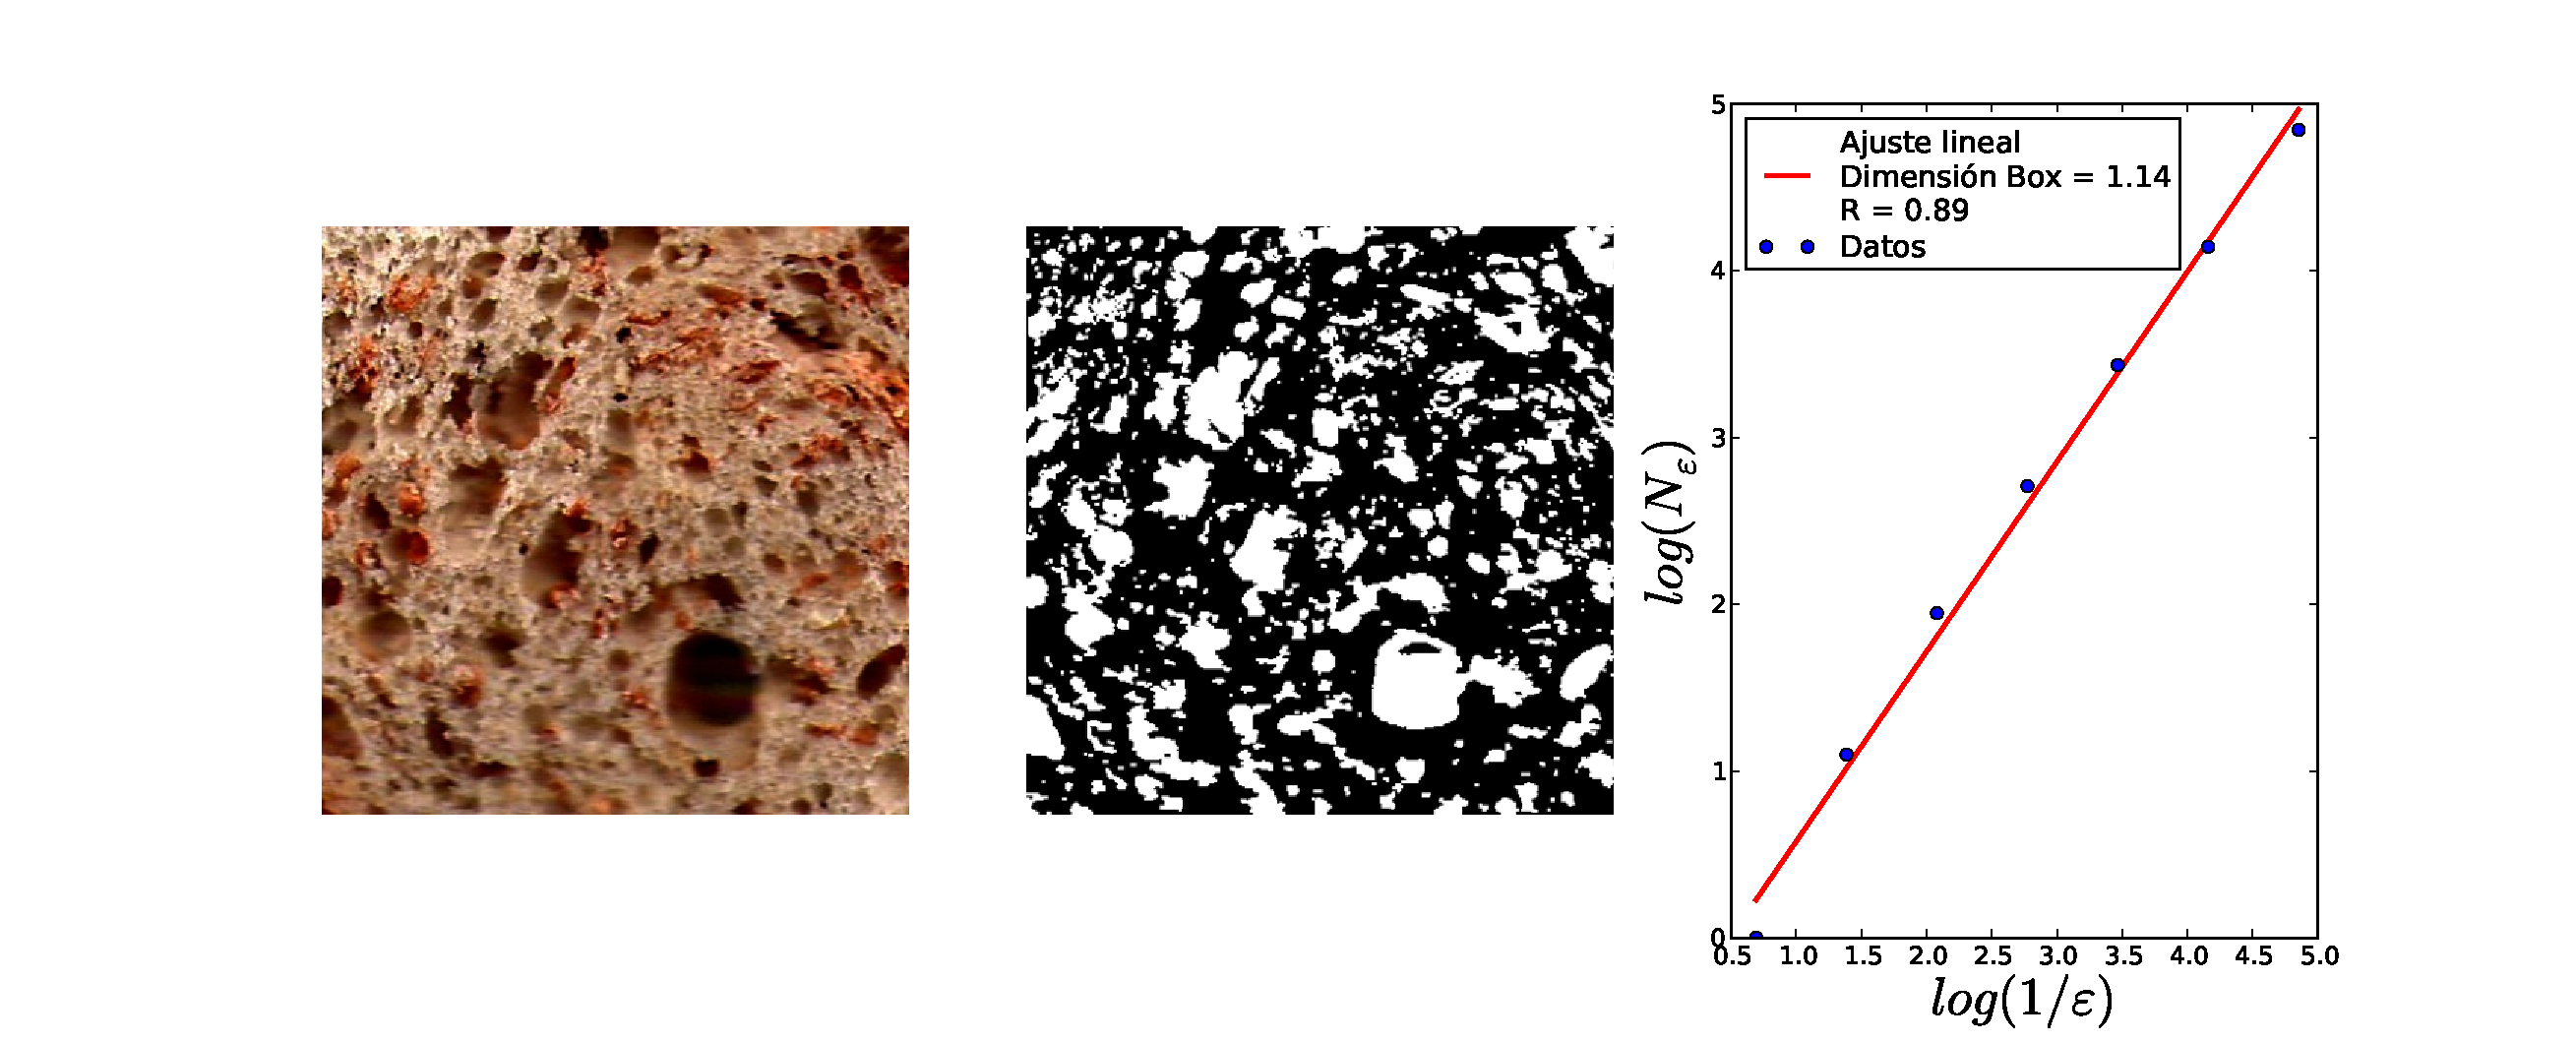
\includegraphics[width=13cm]{dimensionbox}
\caption{Box dimension computation. A bread image (left) with its binarisation (centre) and its computed box dimension (right).}
\label{fig:fitbox}
\end{figure}

\begin{figure}[h!]
\centering
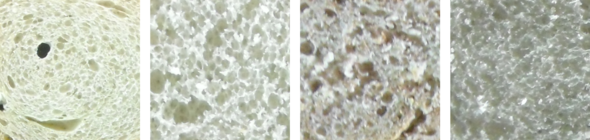
\includegraphics[width=13cm]{pancamara}
\caption{Images from a digital camera.}
\label{fig:camera}
\end{figure}

\begin{figure}[h!]
\centering
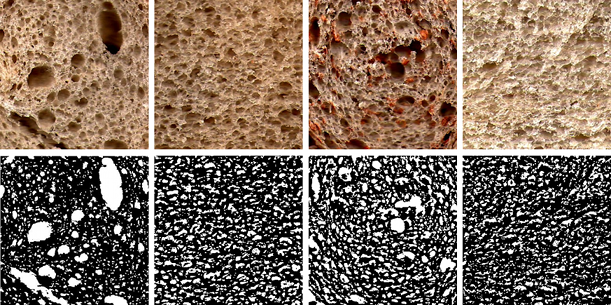
\includegraphics[width=13cm]{binarizaciones}
\caption{Images from a scanner. {\em Baguette}, {\em sliced}, {\em bran} and {\em sandwich} bread types (top row) with their corresponding binarisations (bottom row).}
\label{fig:bread}
\end{figure}

\begin{figure}[h!]
\begin{centering}
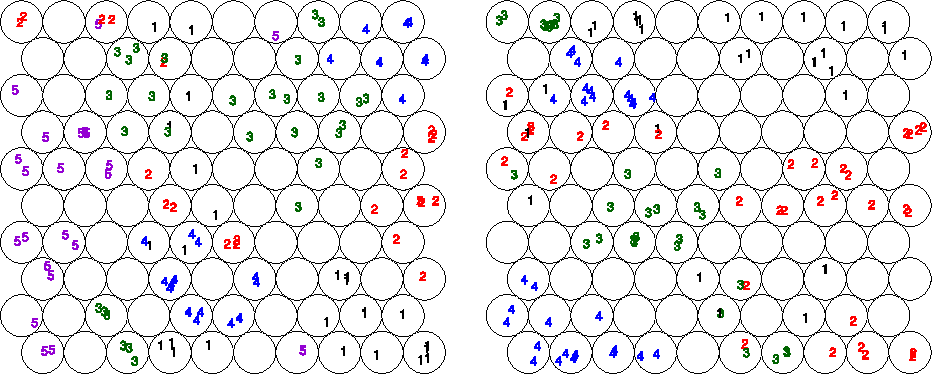
\includegraphics[width=13cm]{SOM}
\caption{Self-organising maps (SOM). SOM of the bread and non-bread images (left) and SOM of the bread types only (right). $1$: {\em baguette}, $2$: {\em sliced}, $3$: {\em bran}, $4$: {\em sandwich}, $5$: {\em nonbread}.}
\label{fig:somfractal}
\end{centering}
\end{figure}

\begin{figure}[h!]
\centering
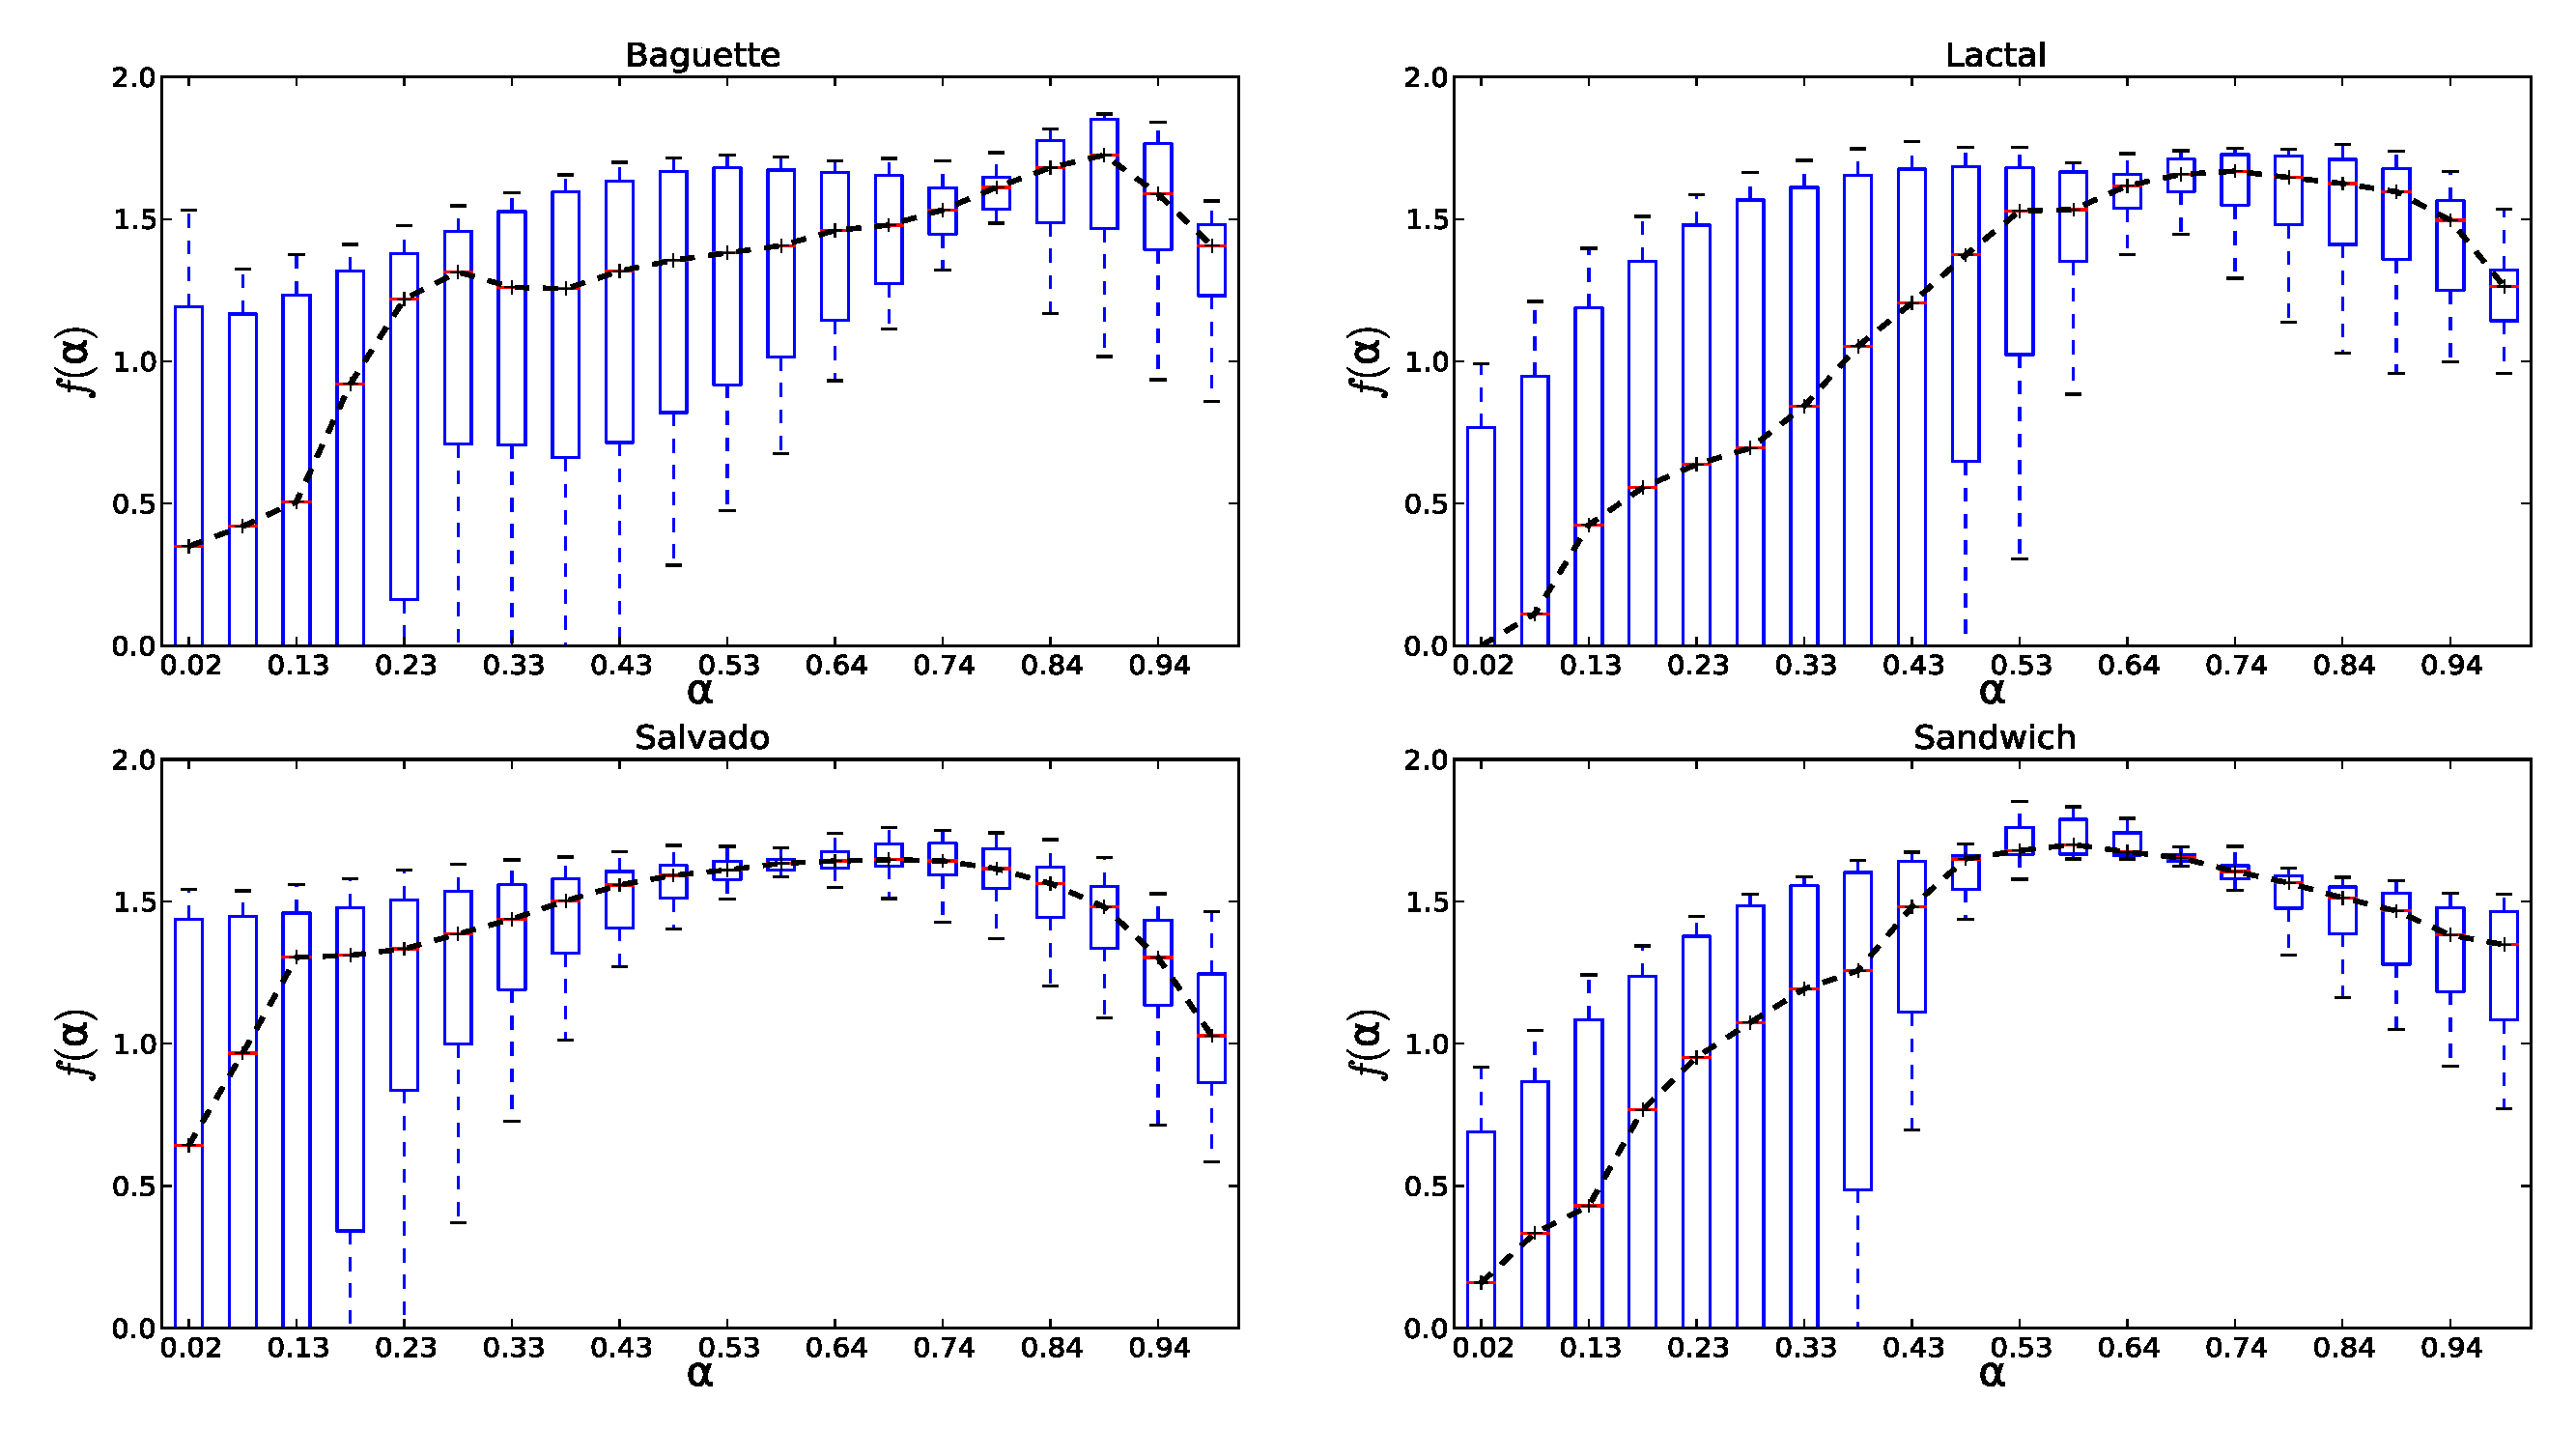
\includegraphics[width=13cm]{boxplots}
\caption{Boxplots of the four different bread types. The FD medians are joined by a dashed line. Top: {\em baguette} (left), {\em sliced} (right), bottom: {\em bran} (left), {\em sandwich} (right).}
\label{fig:boxplotsMFS}
\end{figure}

\begin{figure}[h!]
\centering
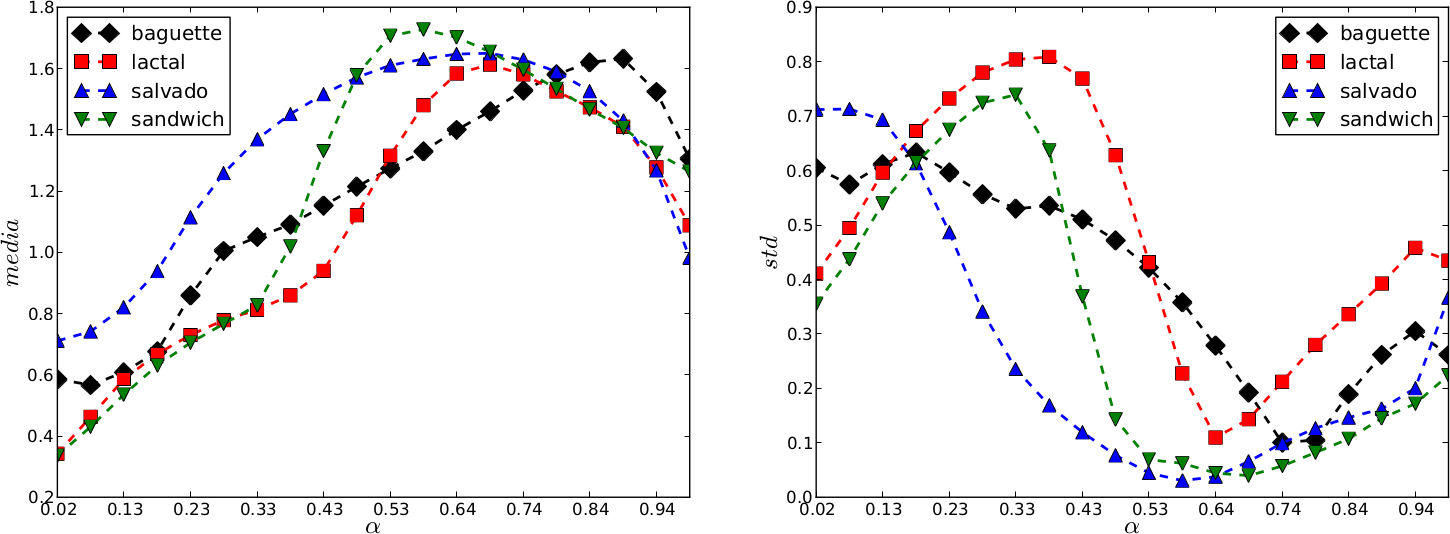
\includegraphics[width=13cm]{panstd}
\caption{Mean MFS and standard deviations of the FDs for the four different bread types. Left: mean MFS, right: standard deviations.}
\label{fig:meansMFS}
\end{figure}


\begin{figure}[h!]
\centering
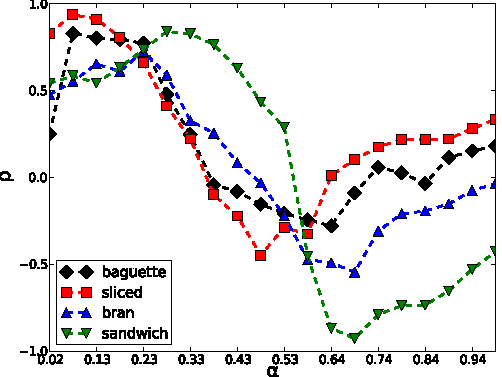
\includegraphics[width=8cm]{VF}
\caption{Spearman correlation coefficients for the FDs and the void fraction of the scanned samples.}
\label{fig:corrVF}
\end{figure}

\begin{figure}[h!]
\centering
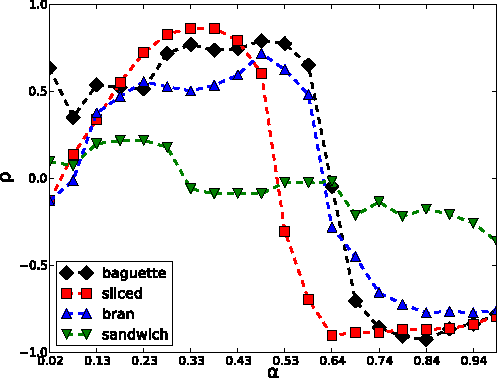
\includegraphics[width=8cm]{MCA}
\caption{Spearman correlation coefficients for the FDs and the mean cell area. (In $[mm^{2}]$, scanned samples).}
\label{fig:corrMCA}
\end{figure}

\begin{figure}[h!]
\centering
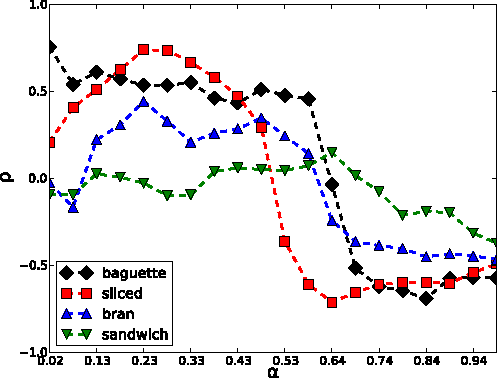
\includegraphics[width=8cm]{stMCA}
\caption{Spearman correlation coefficients for the FDs and the standard deviation of the mean cell area. (In $[mm^{2}]$, scanned samples).}
\label{fig:corrMCAstdev}
\end{figure}




\begin{table}[h!]
\center
% table caption is above the table
\caption{Bread crumb classification results with different number of FDs for the MFS and different classifiers.}
\label{tab:number}       % Give a unique label
% For LaTeX tables use
\begin{tabular}{lllll}
\hline\noalign{\smallskip}
\#FDs & 10  & 20 & 30 \\
\noalign{\smallskip}\hline\noalign{\smallskip}
SVM & \textbf{96\%} & 94.5\% & 95.5\% \\
RF  & 91.5\% & \textbf{93.5\%} & 93\% \\
NN & 88.5\% & \textbf{90.5\%} & 90\% \\
\noalign{\smallskip}\hline
\end{tabular}
\end{table}


\begin{table}[h!]
\center
% table caption is above the table
\caption{Bread crumb classification results using different combinations of the MFS and different classifiers.}
\label{tab:mfs}       % Give a unique label
% For LaTeX tables use
\begin{tabular}{lllll}
\hline\noalign{\smallskip}
Method & MFS & MFS+L & MFS+G & CIELab  \\
\noalign{\smallskip}\hline\noalign{\smallskip}
SVM & 94.5\% & 95.5\% & \textbf{97.5\%} & \textbf{97.5\%} \\
RF  & 93.5\% & \textbf{96\%} & 95\% & \textbf{96\%} \\
NN & 90.5\% & 90\% & 87\% & \textbf{92\%} \\
\noalign{\smallskip}\hline
\#FDs & 20 & 40 & 40 & 60 \\
\hline
\end{tabular}
\end{table}

\begin{table}[h!]
\center
% table caption is above the table
\caption{Bread crumb classification results for different state-of-the-art features and different classifiers.}
\label{tab:other}       % Give a unique label
% For LaTeX tables use
\begin{tabular}{llllll}
\hline\noalign{\smallskip}
Method & Haralick & Lbp & SIFT\\ % & Zernicke
\noalign{\smallskip}\hline\noalign{\smallskip}
SVM & 94\% & 78.5\% & \textbf{96.5\%} \\ % & 55 
RF  & 91\% & 71.5\% & \textbf{92\%} \\ % & 58 
NN & 79\% & 70\% & \textbf{86\%} \\ % & 48.5 
\noalign{\smallskip}\hline
\#FDs & 13 & 36 & 128 \\
\hline
\end{tabular}
\end{table}

\begin{table}[h!]
\center
% table caption is above the table
\caption{Confusion Matrix for the best results (CIELab method, using the SVM classifier).}
\label{tab:confusionmatrix}       % Give a unique label
% For LaTeX tables use
\begin{tabular}{llllll}
\hline\noalign{\smallskip}
Clase&{\em baguette} & {\em lactal} & {\em salvado} &{\em sandwich}&{\em no-pan} \\
\noalign{\smallskip}\hline\noalign{\smallskip}
{\em baguette} & 39& 1 &1 &0 &0 \\
{\em lactal} & 0& 38 &0 &0 &0  \\
{\em salvado} & 0& 0 &39 &1 &0  \\
{\em sandwich} & 1& 1 &0 &39 &0  \\
{\em no-pan} & 0& 0 &0 &0 &40  \\
\hline
\end{tabular}
\end{table}


\section{Validación de Imágenes Sintéticas de Pan}

This section is included for the sole purpose of having a more objective assessment of our model's quality, apart from what subjective inspection may indicate. 
We validated our model using multifractal features, in particular, the multifractal spectrum method, that is widely used for texture analysis in computer vision and pattern analysis.
Fractal Dimensions (FD) can be used to characterize key image features using just a few parameters. 
Different FDs capture different features, {\em e.g.}, porosity, rugosity, etc.
Multifractal theory has also been used for image feature description, but not much in bread characterization. 
A few previous studies show fractal bread characterizations using several FDs \cite{Gonzales2008,Baravalle2012}. 
There are two main classes of multifractal spectra: generalized multifractal dimensions ($D_{q}$) and Lipschitz-H\"older exponents ($f(\alpha)$). 
The latter representation boosts the performance in classification tasks.

The generalized multifractal dimensions can be computed in several ways, of which the Sandbox multifractal method \cite{Tel1989} aims to compute the dimensions using the mean value in a set of randomly distributed points belonging to the structure \cite{Debartolo2004}. 
The generalized multifractal dimension of order $q$ with the sandbox method is defined as:

 \begin{align*}
D_{q\ne 1}^{sb} &= \frac{1}{q-1} \lim_{R \rightarrow 0}{
\frac{ln   { \left\langle  (M(R)/M_{0})^{q-1} \right\rangle   }}
{ln {(R/L)}       }},\\
D_{q=1}^{sb} &= \lim_{R \rightarrow 0}{
\frac{ \left\langle ln   { (M(R)/M_{0})  }  \right\rangle}
{ln {(R/L)}       }},
\end{align*}
%
where $M_{0}$ is the white pixel-count in the image binarization and  $M(R)$ is the number of points belonging to the structure in a circle of radius $R$ centered at a point in the structure. 
When $q\ne1$, we compute the limit as the slope of the linear fit of the values $ln(R/L)$ vs. $ ln  \left\langle  { (M(R)/M_{0})^{q-1} }  \right\rangle$, for $R$ in $[R_{min}, R_{max}]$, where $ \left\langle \cdot  \right\rangle$ denotes mean value over sampled points. 
The proceeding is similar when $q=1$. 
Computing the value for different $q \in [Q_{\min},Q_{\max}]$  we obtain the sandbox spectrum. %We will apply the sandbox approach to characterize real and synthetic bread binarizations.

This kind of analysis is reported to be the most adequate for geometrical and texture feature analysis~\cite{Gonzales2008,Baravalle2012}, so we applied it to $10$ binarized scanned real bread crumb images of the {\em baguette} bread type, and $10$ synthetic images produced using our pipeline, after the baking step, obtaining $20$ feature vectors.
We then separated each class and we computed boxplots for the two classes.
Actual bread crumbs were manually segmented to prevent errors from automatic segmentation as in \cite{Bosch2011}.
The model has $5$ parameters:

\begin{align*}
N &= \frac{k}{r^{d}},\\ r &= v_{min}+step*j, j \in [0,\frac{v_{max}}{step}],
\end{align*}
$k,d,v_{min},v_{max}$ and $step$ that controls bubble generation in the proving stage.
To compute the sandbox spectrum of each image, we used $1000$ different random points to ensure stability in the resulting spectrum.

We implemented an automated search in parameter space defining an error metric: 
\begin{equation*}
Error = \displaystyle \sum abs(means_{real}-means_{synthetic}),
\end{equation*}
and we found that the following parameters produce the lowest error:
\begin{align*}
k &= 0.07 \frac{N^{3}}{20} ,\\
d &=2.78,\\
v_{min} &=2,\\
v_{max} &=20.\\
step &=1,
\end{align*}
where $N$ is the proving volume dimensions in each spatial coordinate (we chose $N = 512$). 
The accumulated error in medians is $\sim 0.21$ meaning a mean error of $0.21/21 \sim 0.01$ in each dimension.
Fig.~\ref{bestboxplot} shows boxplots of real and synthetic breads with the medians for each dimension joined by dashed lines.
When $q < 0$ dimensions have a higher dispersion, since the method approximates these dimensions less accurately.
The figure shows almost identical spectra for real and synthetic breads. Fig.~\ref{realbin} and Fig.~\ref{best} show an example of real and synthetic binarizations for these parameters.


\begin{figure}[!ht]
\includegraphics[width=9cm]{figures/bestboxplot}
\caption{Best fitting parameters for the {\em baguette} bread type. The total error in medians is $\sim 0.21$.}
\label{bestboxplot}
\end{figure}

\begin{figure}[!ht]
\begin{center}
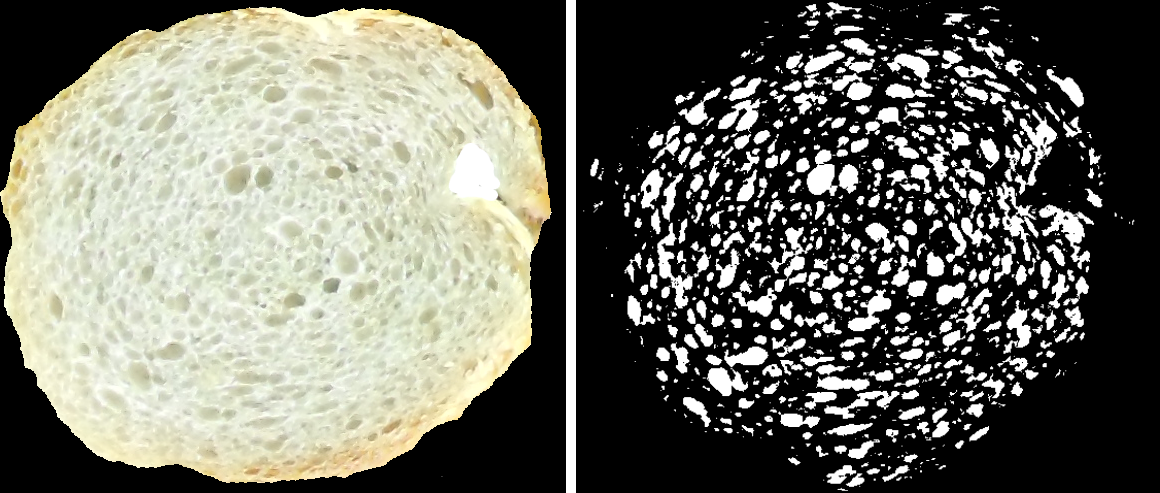
\includegraphics[width=13cm]{figures/realbin}
\caption{ Real {\em baguette} bread and binarization example.}
\label{realbin}
\end{center}
\end{figure}

\begin{figure}[!ht]
\begin{center}
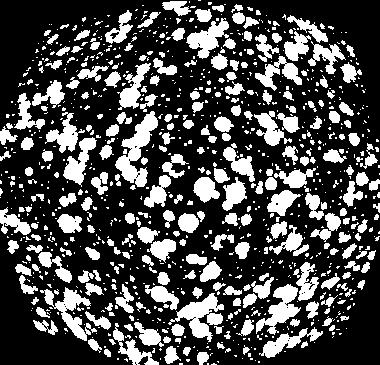
\includegraphics[width=8cm]{figures/best}
\caption{Model distribution example showing similar multifractal features to the {\em baguette} real bread type.}
\label{best}
\end{center}
\end{figure}

Also, we found parameters for a home-baked bread type using the same search:

\begin{align*}
k &= 0.69 \frac{N^{3}}{20} ,\\
d &=5.6,\\
v_{min} &=1,\\
v_{max} &=24.\\
step &=1,
\end{align*}

Fig.~\ref{bestboxplot2} shows boxplots of real and synthetic breads for this bread type. Fig.~\ref{realbin2} and  Fig.~\ref{best2} show an example of real and synthetic binarizations for these parameters and bread type. 


\begin{figure}[!ht]
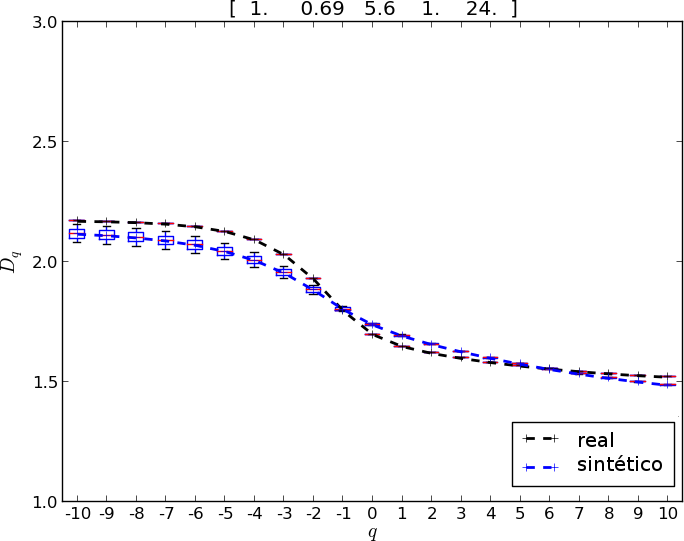
\includegraphics[width=9cm]{figures/bestboxplot2}
\caption{Best fitting parameters for a home-baked bread type. The total error in medians is $\sim 0.88$.}
\label{bestboxplot2}
\end{figure}

\begin{figure}[!ht]
\begin{center}
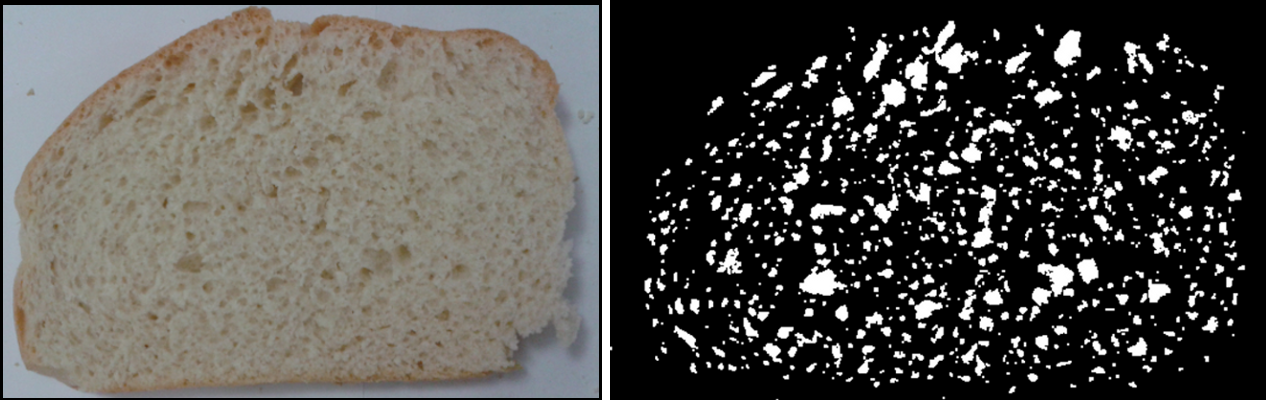
\includegraphics[width=9cm]{figures/realbin2}
\caption{ Real home-baked bread and binarization example.}
\label{realbin2}
\end{center}
\end{figure}

\begin{figure}[!ht]
\begin{center}
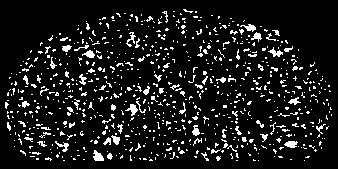
\includegraphics[width=6cm]{figures/best2}
\caption{Model distribution example showing similar multifractal features to a home-baked real bread type.}
\label{best2}
\end{center}
\end{figure}


%We apply the sandbox multifractal method to study the geometry we obtained after the deformation step. This method is best suited for geometrical measurements than other multifractal approaches.

%We apply the sandbox method to $10$ binarised real bread crumb images of the {\em baguette} bread type that we captured with a digital scanner and $10$ syhthetic images produced using our pipeline, after the deformation step, obtaining $20$ feature vectors. Then we separate each class and we compute boxplots for the two classes. We manually segmented real bread crumbs to prevent automatic segmentation errors as in \cite{Bosch2011}. The model has $5$ parameters:


%\begin{align}
%N_{spheres} &= \frac{k}{r^{d}},\\ r &= v_{min}+step*j, j \in [0,\frac{v_{max}}{step}]
%\end{align}
%$k,d,v_{min},v_{max}$ and $step$ that controls bubble's generation in the proving stage. %To compute the sandbox spectrum of each image, we used $5000$ different random points to ensure stability in the resulting spectrum.

%We implemented an automated search in parameter space and we found that the following parameters produce the lowest error:

%\begin{align*}
%k &= 0.07 \frac{N_{x}\times N_{y}\times N_{z}}{20} ,\\
%d &=2.78,\\
%v_{min} &=2,\\
%v_{max} &=20.\\
%step &=1,
%\end{align*}
%\noindent where $N_{x}$, $N_{y}$ and $N_{z}$ are the proving volume dimensions in each spatial coordinate (we chose $(N_{x},N_{y},N_{z}) = (760,760,100)$). The accumulated error in medians is $\sim 0.21$ meaning a mean error of $0.21/21 \sim 0.01$  in each dimension. We compute this error as:

%\begin{equation}
%Error = \displaystyle \sum abs(means_{real}-means_{synthetic}).
%\end{equation}
%Fig.~\ref{bestboxplot} shows boxplots of real and synthetic breads with the medians for each dimension joined by dashed lines. When $q < 0$ dimensions have a higher dispersion, since the method approximates these dimensions less accurately. The figure shows almost identical spectra for real and synthetic breads.  Fig.~\ref{realbin} and  Fig.~\ref{bestwarp} show an example of real and synthetic binarisations for these parameters.

%\begin{figure}[!ht]
%\includegraphics[scale=0.5]{bestboxplot.png}
%\caption{Best fitting parameters. The total error in medians is $\sim 0.21$.}
%\label{bestboxplot}
%\end{figure}

%\begin{figure}[!ht]
%\begin{center}
%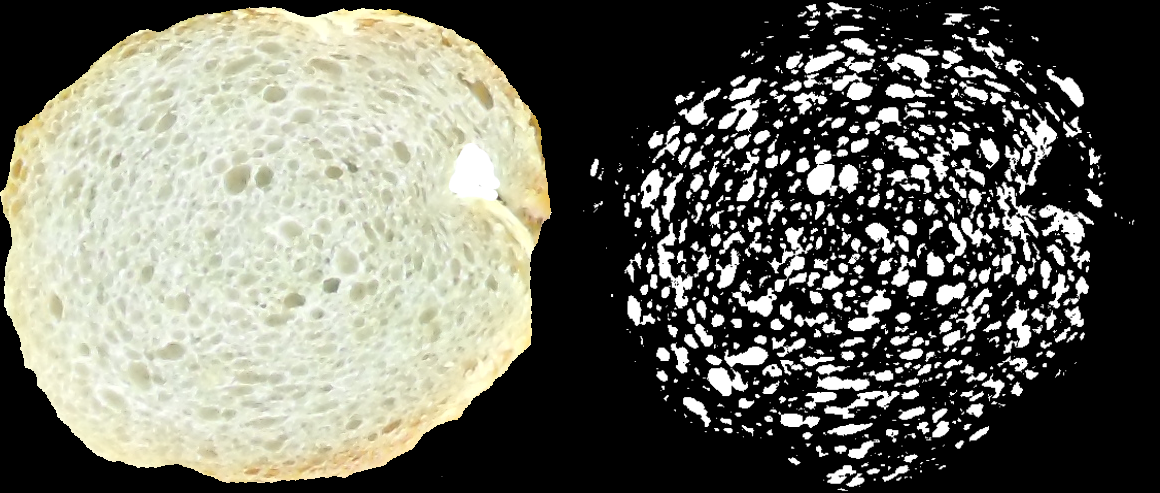
\includegraphics[scale=0.2]{realbin.png}
%\caption{ Real bread and binarisation example.}
%\label{realbin}
%\end{center}
%\end{figure}

%\begin{figure}[!ht]
%\begin{center}
%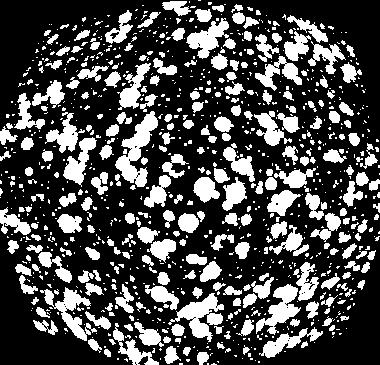
\includegraphics[scale=0.4]{bestwarp.png}
%\caption{Model distribution example showing similar multifractal features to real breads .}
%\label{bestwarp}
%\end{center}
%\end{figure}


%Automated searchs in parameter space may be useful to automatically match other bread types and materials.

%\section{Resultados}

\section{Validación utilizando técnicas de Aprendizaje Profundo}

\section{Discusión y Conclusiones}

The visual appearance of different types of bread crumbs can be successfully characterised by the multifractal dimensions of their digital images. The FDs obtained from the MFS method whose $\alpha \in [0,0.23]$ provided a good measure of the bread crumb porosity, meaning that the higher these FDs, the higher the measure. In addition, the FDs whose $\alpha \in [0.79,1]$ are useful to measure coarseness and heterogeneity of bread crumb. The MFS contains useful data to characterise the three measures, combining the information in one feature vector.

The use of multifractal features in bread crumb texture classification showed excellent performance. The MFS de\-monstrated to be accurate enough to perform a classification of different bread types and also to discriminate non bread from bread images. The classification performance of the MFS for the bread crumb database outperforms other state-of-the-art techniques employed in the computer vision literature. The information present in the MFS of the $L$, $a$ and $b$ channels of the CIElab space colour obtained the best classification performance in all the developed tests. This result appears to be a consequence of the different capturing devices used in this work. Also, it was shown that the MFS is sensitive to changes in the illumination conditions during image acquisition.

The sandbox multifractal method allows to approximate the geometry of any real bread crumb, by 
extracting parameters in order to accurately simulate it.
Bubble distributions under our model were shown to be statistically coincident to real bread, according to multifractal methods.
The sandbox analysis method produced very similar fractal features both with our synthetic images and with images of real bread crumbs.
Two bread types were tested: a home-baked and the {\em baguette } bread types.
The home-baked multifractal spectrum was more difficult to fit ({\em i.e.}, the errors were larger than those of the {\em baguette} bread type), but notwithstanding this the final bubble distribution was adequate for emulating this bread type.
Multifractal spectra showed higher dispersion in the negative dimensions ($q < 0$), which means that at finer geometric scales it is more difficult to characterize the statistical distribution, due to the image resolution.
A more detailed link between bread crumb physical features (coarseness, porosity) and multifractal features may be useful for designing better procedural models \cite{Baravalle2012}.
Multifractal image analysis was used to validate the model.
The statistical similarity between $2D$ cuts in our results and of real-word bread slices suggests that it may be suitable for applications in $3D$ engines, serious games \cite{Susi2007} and photorealistic rendering. 

%citar imfractal


